\chapter{Pruebas y resultados}
\label{chap:pruebas}
\section{Análisis del entrenamiento de la segmentación semantica}
\subsection{Descripción de los equipos}
Se realizo los entrenamientos con diferentes configuraciones, las especificaciones del equipo utilizado para el entrenamiento son: 
\begin{itemize}
    \item Procesador
    \begin{itemize}
        \item Nombre del Modelo: Intel(R) Core(TM) i7-5930K CPU @ 3.50GHz
        \item Frecuencia maxima:  3700.0000 MHz
     \item Frecuencia minima: 1200.0000 MHz
     \item Arquitectura :  x86\_64
     
    \end{itemize}{}
    \item Tarjeta de video
    \begin{itemize}
        \item Nombre del Modelo: GeForce GTX 1080
        \item Memoria : 8119 MiB
        \item Cantidad : 3
        \item Nucleos Cuda por tarjeta : 2560
        \item Frecuencia base : 1607 
        
    \end{itemize}{}
    \item Memoria RAM : 62 GB 
\end{itemize}{}
Las especificaciones del equipo en CPU fueron :
\begin{itemize}
    \item Memoria : 48 GB
    ·   \item Procesador
    \begin{itemize}
        \item Nombre del Modelo:  Intel(R) Core(TM) i7-7700 CPU @ 3.60GHz
        \item Frecuencia maxima: 4200,0000 MHz
     \item Frecuencia minima: 800,0000 MHz
     \item Arquitectura :  x86\_64
     
    \end{itemize}{}
    

\end{itemize}{}
\subsection{Parámetros de Red}
  \begin{table}[H]
      \centering
            \caption{Parámetros de entrenamiento Redes Neuronales}

      \begin{tabular}{|c|c|} \hline
          Parametro & Cantidad  \\\hline
           Tamaño Batch &   10 \\
           Workers & 3 \\
           Learnign rate  & 0.0008\\
           Optimizador & AdamW \\
           Tamaño Original & 256 \\
           Imágenes Entrenamiento sin Aumento de Data & 1296 \\
           
           Técnicas de aumento de data usados  & 9 \\
           Imágenes de Test & 240 \\\hline
           
           
           
           
           
      \end{tabular}
      \label{tab:my_label}
  \end{table}{}


\subsection{Análisis de funciones de perdida}

\begin{figure}[H]
    \centering
    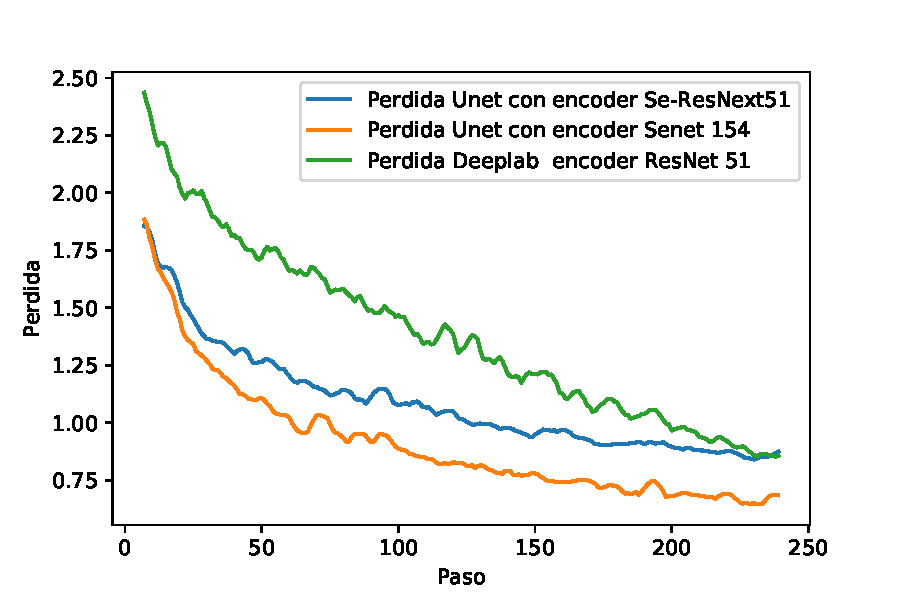
\includegraphics[width=0.8\textwidth]{images/funciones/comparacionesLos.pdf}
    \caption{Gráfica representando la función de perdida de las Redes Neuronales}
    \label{fig:graficasPerdida}
\end{figure}{}

De la \figurename~\ref{fig:graficasPerdida} se puede concluir lo siguiente :
\begin{itemize}
    \item Cuando se utiliza un encoder más profundo la red neuronal tiende a llegar a un punto de equilibrio más rápido.
    \item Si bien las redes neuronales aun no han llegado a un punto de equilibrio, este se tomo como valido.
\end{itemize}{}


\subsection{Análisis de \gls{Accuracy}}

\begin{figure}[H]
    \centering
    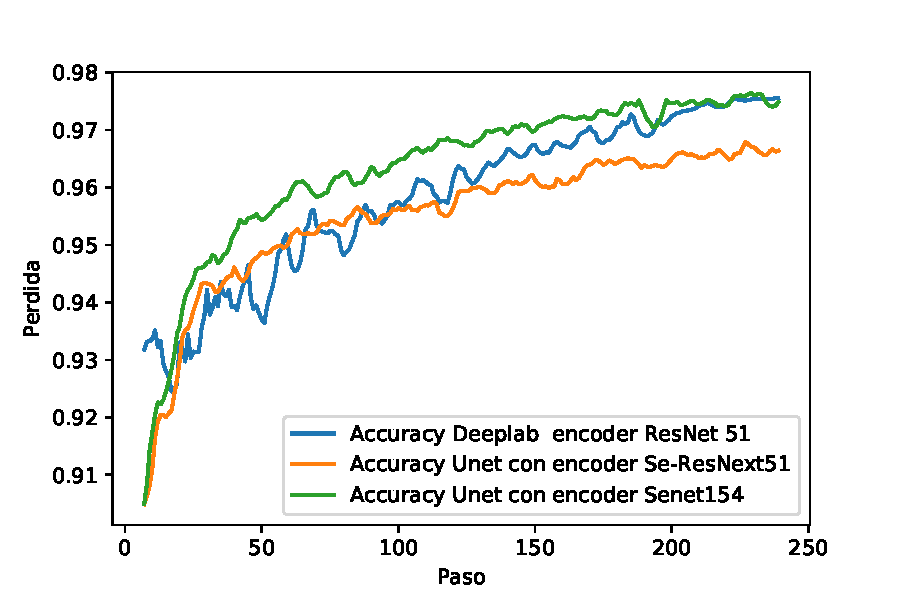
\includegraphics[width=0.8\textwidth]{images/funciones/comparacionesAcc.pdf}
    \caption{Gráfica representando la \gls{Accuracy} de las Redes Neuronales}
    \label{fig:Accuracy}
\end{figure}{}
En la \figurename~\ref{fig:Accuracy} se aprecia el progreso del \gls{Accuracy} a través de iteraciones, de esto se puede deducir lo siguiente 
\begin{itemize}
    \item Una red con un Encoder menos profundo tiende a tener peores resultados.
    \item Una correcta arquitectura de red Neuronal puede lograr obtener mejores resultados con una menor cantidad de capaz.
\end{itemize}

\section{Análisis de evaluación en los datos de test}
\begin{table}[H]
    \centering
        \caption{Tabla de \gls{Accuracy} de cada modelo}

    \begin{tabular}{|c|c|}
    \hline  Red Neuronal  &  \gls{Accuracy}   \\ \hline
         Deeplab ResNext 51   &  0.9883300781		\\
        Unet ResNext 51& 0.9923184482	 \\	
        Unet SeNet154 & 0.9923661665	\\	
   Unet   & 0.9849744524 \\  \hline
    \end{tabular}
    
    \label{tab:Acuracy}
\end{table}{}
\begin{table}[H]
    \centering
    \caption{Tiempo de ejecución de la red neuronal en la computadora de solo CPU}
    \begin{tabular}{|c|c|}
  \hline  Red neuronal & Imágenes por Segundo \\ \hline
        Deeplab ResNext 51&		7.8 \\
Unet	&	8.04 \\
  Unet ResNext 51	&	2.98 \\ 
 Unet SeNet154	&	1.2 \\
 \hline
          
    \end{tabular}
    \label{tab:tablaTiemposCPU}
\end{table}{}
Los resultados del \tablename \ref{tab:tablaTiemposCPU} fueron obtenidos luego de promediar 3 ejecuciones con un tamaño de base de datos de 240 imágenes.
\begin{table}[H]
    \centering
    \caption{Tiempo de ejecución de la red neuronal en la computadora de GPU}
    \begin{tabular}{|c|c|}
  \hline  Red neuronal & Imágenes por Segundo \\ \hline
     Deeplab ResNext 51&	72.26 \\
Unet	&	66.77 \\
  Unet ResNext 51	&	51.26\\ 
 Unet seNet154	&	24.27\\
 \hline
          
    \end{tabular}
    \label{tab:tablaTiemposGPU}
    \end{table}{}

Los resultados del \tablename \ref{tab:tablaTiemposGPU} fue el resultado de promediar los tiempo
\subsection{Resultados Segmentación Semántica}

Como resultado final se puede ver algunas de la imágenes procesadas son:

\begin{table}[H]
\caption{Resultados de Segmentación Semántica }

\begin{tabular}{|M{0.3\textwidth}|M{0.3\textwidth}|M{0.3\textwidth}|}
 \hline Original & Obtenida & Binarizada por umbral \\
 \hline
\medskip  \fbox{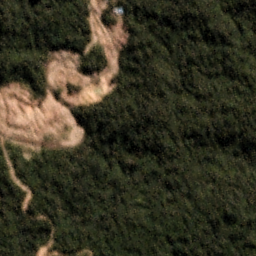
\includegraphics[width=0.25\textwidth]{images/datos/train80047.png}}
 &\medskip \fbox{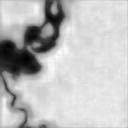
\includegraphics[width=0.25\textwidth]{images/datos/outfileSinBinarizar90001.png}}
  & \medskip\medskip \fbox{
\includegraphics[width=0.25\textwidth]{images/datos/outfileBinarizado90001.png}}
  
  \\

 \medskip \fbox{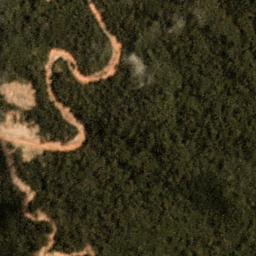
\includegraphics[width=0.25\textwidth]{images/datos/train70047.png}} \medskip 
 &\medskip \fbox{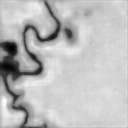
\includegraphics[width=0.25\textwidth]{images/datos/outfileSinBinarizar90000.png}} \medskip 
  &\medskip \fbox{
\includegraphics[width=0.25\textwidth]{images/datos/outfileBinarizado90000.png}} \medskip 
\\
\hline

\end{tabular}
\label{table:resultadosSegmentacion}
\end{table}

En los resultados mostrados en le \tablename~\ref{table:resultadosSegmentacion}, la columna sin binarizar muestra la segmentación en escala de grises donde el blanco más intenso en un píxel significa mayor posibilidad a que este pixel sea un árbol.
\begin{table}[H]
\caption{Resultados de Segmentación Semántica }

\begin{tabular}{|M{0.19\textwidth}|M{0.19\textwidth}|M{0.19\textwidth}|M{0.19\textwidth}|M{0.19\textwidth}|}
 \hline Original & Unet Clasica& Unet-ResNext 51 &  Unet-Senet154 & Deeplab \\
 \hline
\medskip  \fbox{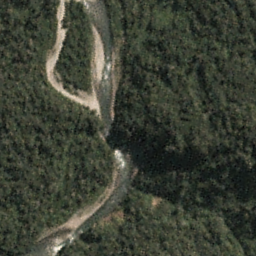
\includegraphics[width=0.15\textwidth]{images/imagenesEjemplo/6/img.png}}
 &\medskip \fbox{
\includegraphics[width=0.15\textwidth]{images/imagenesEjemplo/6/unet.png}}
  & \medskip\medskip \fbox{
\includegraphics[width=0.15\textwidth]{images/imagenesEjemplo/6/unet51.png}}
    & \medskip\medskip \fbox{
\includegraphics[width=0.15\textwidth]{images/imagenesEjemplo/6/unet154.png}}
      & \medskip\medskip \fbox{
\includegraphics[width=0.15\textwidth]{images/imagenesEjemplo/6/deeplab.png}}
  \\
\medskip  \fbox{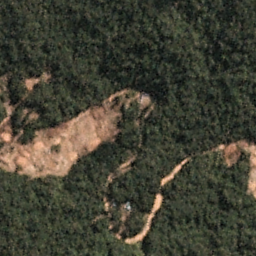
\includegraphics[width=0.15\textwidth]{images/imagenesEjemplo/5/img.png}}
 &\medskip \fbox{
\includegraphics[width=0.15\textwidth]{images/imagenesEjemplo/5/unet.png}}
  & \medskip\medskip \fbox{
\includegraphics[width=0.15\textwidth]{images/imagenesEjemplo/5/unet51.png}}
    & \medskip\medskip \fbox{
\includegraphics[width=0.15\textwidth]{images/imagenesEjemplo/5/unet154.png}}
      & \medskip\medskip \fbox{
\includegraphics[width=0.15\textwidth]{images/imagenesEjemplo/5/deeplab.png}}
  \\
  \medskip  \fbox{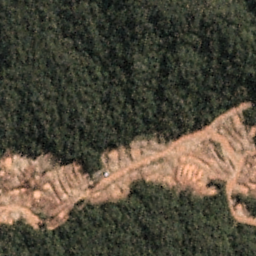
\includegraphics[width=0.15\textwidth]{images/imagenesEjemplo/4/img.png}}
 &\medskip \fbox{
\includegraphics[width=0.15\textwidth]{images/imagenesEjemplo/4/unet.png}}
  & \medskip\medskip \fbox{
\includegraphics[width=0.15\textwidth]{images/imagenesEjemplo/4/unet51.png}}
    & \medskip\medskip \fbox{
\includegraphics[width=0.15\textwidth]{images/imagenesEjemplo/4/unet154.png}}
      & \medskip\medskip \fbox{
\includegraphics[width=0.15\textwidth]{images/imagenesEjemplo/4/deeplab.png}}
  \\
  \medskip  \fbox{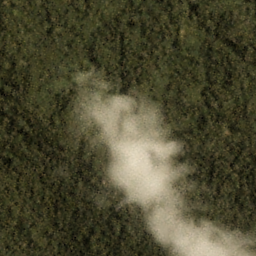
\includegraphics[width=0.15\textwidth]{images/imagenesEjemplo/3/img.png}}
 &\medskip \fbox{
\includegraphics[width=0.15\textwidth]{images/imagenesEjemplo/3/unet.png}}
  & \medskip\medskip \fbox{
\includegraphics[width=0.15\textwidth]{images/imagenesEjemplo/3/unet51.png}}
    & \medskip\medskip \fbox{
\includegraphics[width=0.15\textwidth]{images/imagenesEjemplo/3/unet154.png}}
      & \medskip\medskip \fbox{
\includegraphics[width=0.15\textwidth]{images/imagenesEjemplo/3/deeplab.png}}
  \\
  \medskip  \fbox{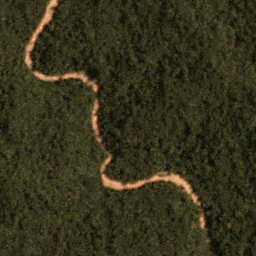
\includegraphics[width=0.15\textwidth]{images/imagenesEjemplo/2/img.png}}
 &\medskip \fbox{
\includegraphics[width=0.15\textwidth]{images/imagenesEjemplo/2/unet.png}}
  & \medskip\medskip \fbox{
\includegraphics[width=0.15\textwidth]{images/imagenesEjemplo/2/unet51.png}}
    & \medskip\medskip \fbox{
\includegraphics[width=0.15\textwidth]{images/imagenesEjemplo/2/unet154.png}}
      & \medskip\medskip \fbox{
\includegraphics[width=0.15\textwidth]{images/imagenesEjemplo/2/deeplab.png}}
  \\
  \medskip  \fbox{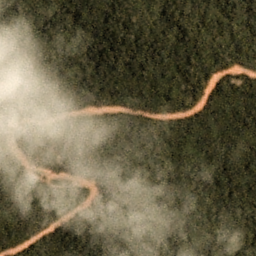
\includegraphics[width=0.15\textwidth]{images/imagenesEjemplo/1/img.png}}
 &\medskip \fbox{
\includegraphics[width=0.15\textwidth]{images/imagenesEjemplo/1/unet.png}}
  & \medskip\medskip \fbox{
\includegraphics[width=0.15\textwidth]{images/imagenesEjemplo/1/unet51.png}}
    & \medskip\medskip \fbox{
\includegraphics[width=0.15\textwidth]{images/imagenesEjemplo/1/unet154.png}}
      & \medskip\medskip \fbox{
\includegraphics[width=0.15\textwidth]{images/imagenesEjemplo/1/deeplab.png}}
  \\

\hline

\end{tabular}
\label{table:resultadosSegmentacion}
\end{table}

\subsection{Resultados de Detección de cambios}
Una vez obtenidos las mascaras de segmentación binarias se procederá a realizar las operaciones descritas en el trabajo de \cite{Doshi2018}. Repitiendo la operación XOR del proceso de detección de cambios. El resultado se aprecia en la siguiente figura.
 
 

\begin{figure}[H]
	\centering
	\begin{tabular}{ccc}
\fbox{	
\includegraphics[width=0.2\textwidth]{images/datos/outfileBinarizado90001.png}} &
\fbox{		
\includegraphics[width=0.2\textwidth]{images/datos/outfileBinarizado90000.png}} &\fbox{
\includegraphics[width=0.2\textwidth]{images/datos/cambio.png}}
	\\
		a) Entrada 1  & b) Entrada 2  & c) Resultado XOR \\						
	\end{tabular}
	\caption{Gráficas que muestra el las entradas y salidas de la operación XOR}

	\label{fig:ResultadosXOR}
\end{figure}



%http://sci-hub.tw/10.1016/j.isprsjprs.2013.03.006